%!TEX TS-program = xelatex
%!TEX encoding = UTF-8 Unicode

\documentclass[12pt,a4paper]{article}
\usepackage{fontspec,xltxtra,xunicode}
\usepackage{fancyhdr}
\usepackage[a4paper,margin=3cm]{geometry}
\setmainfont[Scale=1.22]{TH Sarabun New}
\XeTeXlinebreaklocale 'th_TH'

\author{\sitdhibong}

% Source code
\usepackage{listings}
\lstdefinestyle{sitdhcodelisting}{
    frame=trBL,
    showspaces=false,
    numberstyle=\tiny, 
    language=Java, 
    numbers=left
}

% Graphic
\usepackage{graphicx}
% Multiple row
\usepackage{multirow}
% Table
\usepackage{array}
% Landscape page
\usepackage{pdflscape}
% Title
\usepackage{titleref}

\newcommand{\sitdhibong}{สิทธิพงษ์ เหล่าโก้ก}
\newcommand{\studentid}{5870972621}
\newcommand{\department}{สาขาวิชาวิศวกรรมซอฟต์แวร์}
\newcommand{\faculty}{คณะวิศวกรรมศาสตร์}
\newcommand{\myprogram}{แผน ข. ภาคนอกเวลาราชการ}
\newcommand{\university}{จุฬาลงกรณ์มหาวิทยาลัย}
\newcommand{\subject}{Software Testing and Quality Assurance}
\newcommand{\outbound}{Some input value is out of range}
\newcommand{\nottriangle}{Not a triangle}
\newcommand{\equ}{Equilateral}
\newcommand{\sca}{Scalene}
\newcommand{\iso}{Isoscalene}
\newcommand{\numbername}{ข้อ}
\newcommand{\righttri}{Right triangle}

\renewcommand{\lstlistingname}{รายการที่}
\renewcommand{\figurename}{ภาพที่}
\renewcommand{\tablename}{ตารางที่}

\pagestyle{fancy}
\lhead{\subject}
\rhead{การบ้านครั้งที่ 4: Path testing}
\lfoot{\sitdhibong: \studentid}

% Source code cosmatic
\lstset{columns=fullflexible,basicstyle=\ttfamily}

\begin{document}
%    \section{ข้อมูลทั่วไป}
%    \label{sec:general}
%    \begin{enumerate}
%        \item โปรแกรมตรวจสอบรูปสามเหลี่ยมนี้พัฒนาขึ้นโดยใช้ภาษา JavaScript และใช้ HTML ร่วมกันกับ CSS เพื่อแสดงผล
%        \item สคริปต์ที่พัฒนาขึ้นทั้งหมดอยู่ภายในโฟลเดอร์ path-testing ซึ่งแยกออกเป็น 2 ไฟล์หลัก ได้แก่
%            \begin{itemize}
%                \item {\bf index.html} ซึ่งเรียกไฟล์ asset/js/bundle.js สำหรับโค้ดที่ใช้วาด Control Flow Graph แบบปรกติ
%                \item {\bf index-instrumented.html} ซึ่งเรียกไฟล์ asset/js/bundle-instrumented.js สำหรับตรวจสอบการทำงานของ Test case
%            \end{itemize}
%        \item ไฟล์ JavaScript ที่พัฒนาขึ้นมานี้ทั้ง asset/js/bundle.js และ asset/js/bundle-instrumented.js สำหรับโค้ดแบบปรกติ และโค้ดที่ทำ Instrument แล้ว ตามลำดับ \label{enu:js}
%        \item โค้ดที่นำมาแสดงใน \numbername~\ref{sec:trianglecal}~{\bf \titleref{sec:trianglecal}} คือโค้ดที่มาจากไฟล์ {\bf asset/js/bundle.js} แต่ตัดช่องว่างระหว่างบรรทัดออก เพื่อให้วาด Control Flow Graph ได้กระชับมากยิ่งขึ้น
%        \item วิธีการเรียกใช้งานทำได้ด้วยการเปิดไฟล์ {\bf index-instrumented.html} ที่อยู่ด้านบนสุดของโฟลเดอร์งาน ผ่านเบราว์เซอร์ที่รองรับ เพื่อเริ่มตรวจสอบกรณีทดสอบ
%            \begin{itemize}
%                \item แนะนำ: {\bf Firefox, Safari หรือ Google Chrome เวอร์ชันล่าสุด}
%            \end{itemize}
%        \item สคริปต์ในข้อ~\ref{enu:js} จะใช้งานร่วมกันกับ JavaScript Framework ที่ชื่อว่า jQuery ซึ่งจะรองรับเบราว์เซอร์ดังนี้
%            \begin{itemize}
%                \item Internet Explorer เวอร์ชั่น 9 หรือใหม่กว่า
%                \item Google Chrome เวอร์ชั่นปัจจุบัน
%                \item Firefox เวอร์ชั่นปัจจุบัน
%                \item Safari เวอร์ชัน 5.1 หรือใหม่กว่า 
%                \item Opera เวอร์ชั่นปัจจุบัน 
%                \item iOS เวอร์ชั่น 6.1 หรือใหม่กว่า
%                \item Android เวอร์ชั่น 2.3 และ 4.0 หรือใหม่กว่า
%            \end{itemize}
%    \end{enumerate}
%    \vfill
%    \noindent\sitdhibong\, \studentid \newline
%    \myprogram\, \newline
%    \department\, \faculty
% 
%    \begin{figure}[ht!]
%        \centering
%        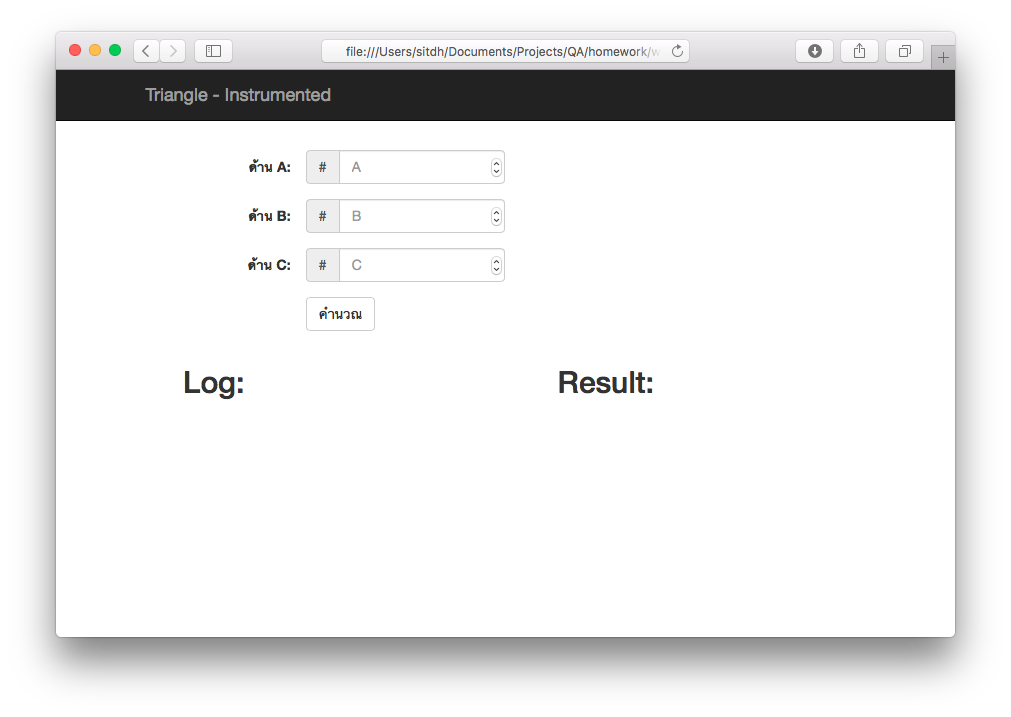
\includegraphics[width=0.9\textwidth]{img/application.png}
%        \caption{หน้าต่างโปรแกรม\label{fig:application}}
%    \end{figure}
% 
%    \begin{figure}[ht!]
%        \centering
%        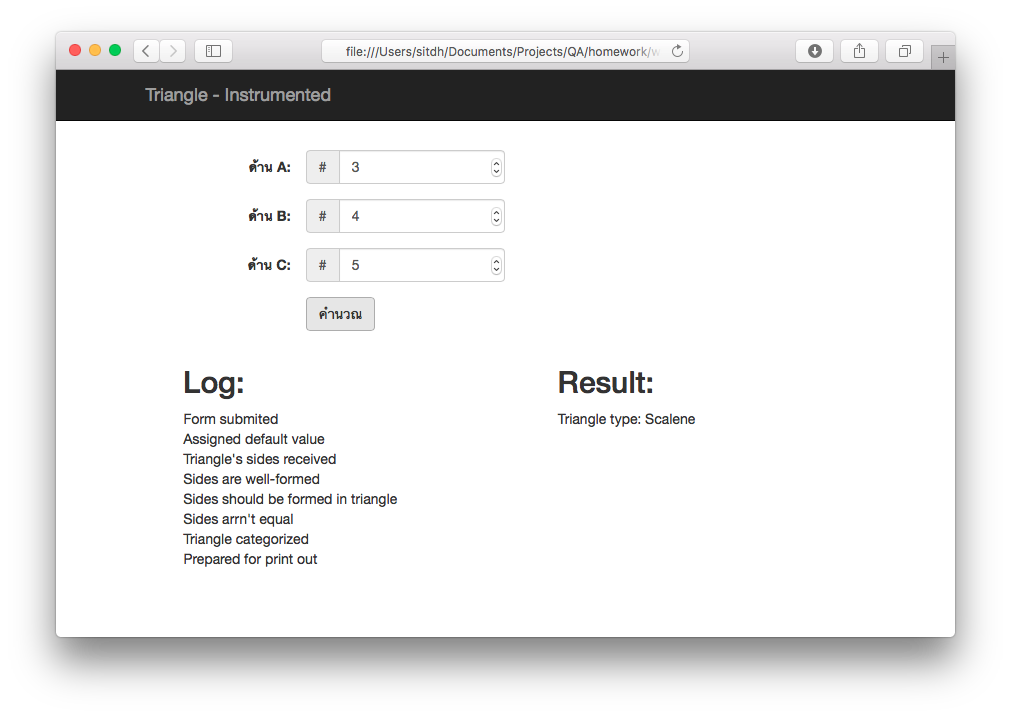
\includegraphics[width=0.9\textwidth]{img/instrumented.png}
%        \caption{หน้าต่างโปรแกรมหลังจากตรวจด้านของรูปสามเหลี่ยมที่นำเข้า\label{fig:instrumented}}
%    \end{figure}
% 
% % Triangle check
% \newpage
% \clearpage
\section[โปรแกรมคำนวณรูปสามเหลี่ยม]{โปรแกรมคำนวณรูปสามเหลี่ยม}
\label{sec:trianglecal}
จากรายการความต้องการเพื่อตรวจสอบรูปสามเหลี่ยม จะนำมาเขียนโปรแกรมด้วยภาษา JavaScript ดังแสดงให้เห็นด้านล่าง
\lstinputlisting[style=sitdhcodelisting, label=lst:trianglecheck lsttitle=\lstname, caption=โปรแกรมตรวจสอบรูปสามเหลี่ยมภาษา JavaScript]{src/compute.js}

% My information
\vfill
\noindent\sitdhibong\, \studentid \newline
\myprogram\, \newline
\department\, \faculty

\newpage
\clearpage
\section[โปรแกรมคำนวณรูปสามเหลี่ยมใส่คำอธิบาย]{โปรแกรมคำนวณรูปสามเหลี่ยมพร้อมใส่โค้ดพิเศษแสดงการทำงาน}
\label{sec:trianglecalinstrumented}
นำโค้ดจาก \numbername~\ref{sec:trianglecal} มาใส่โค้ดพิเศษเพื่อแสดงให้เห็นว่าโปรแกรมได้ทำงานทุกส่วนของโปรแกรม
\lstinputlisting[style=sitdhcodelisting, label=lst:trianglecheckinst title=\lstname, caption=โปรแกรมตรวจสอบรูปสามเหลี่ยมภาษา JavaScript - Instruemented]{src/compute-instrumented.js}

\newpage
% Control flow graph
\clearpage
\section{Control flow graph}
จากโปรแกรมคำนวณรูปสามเหลี่ยมจาก \numbername~\ref{sec:trianglecal} นำมาวาด Control flow graph ได้ดังรูปด้านล่าง

\begin{figure}[h!]
    \label{fig:flowgraph}
    \centering
    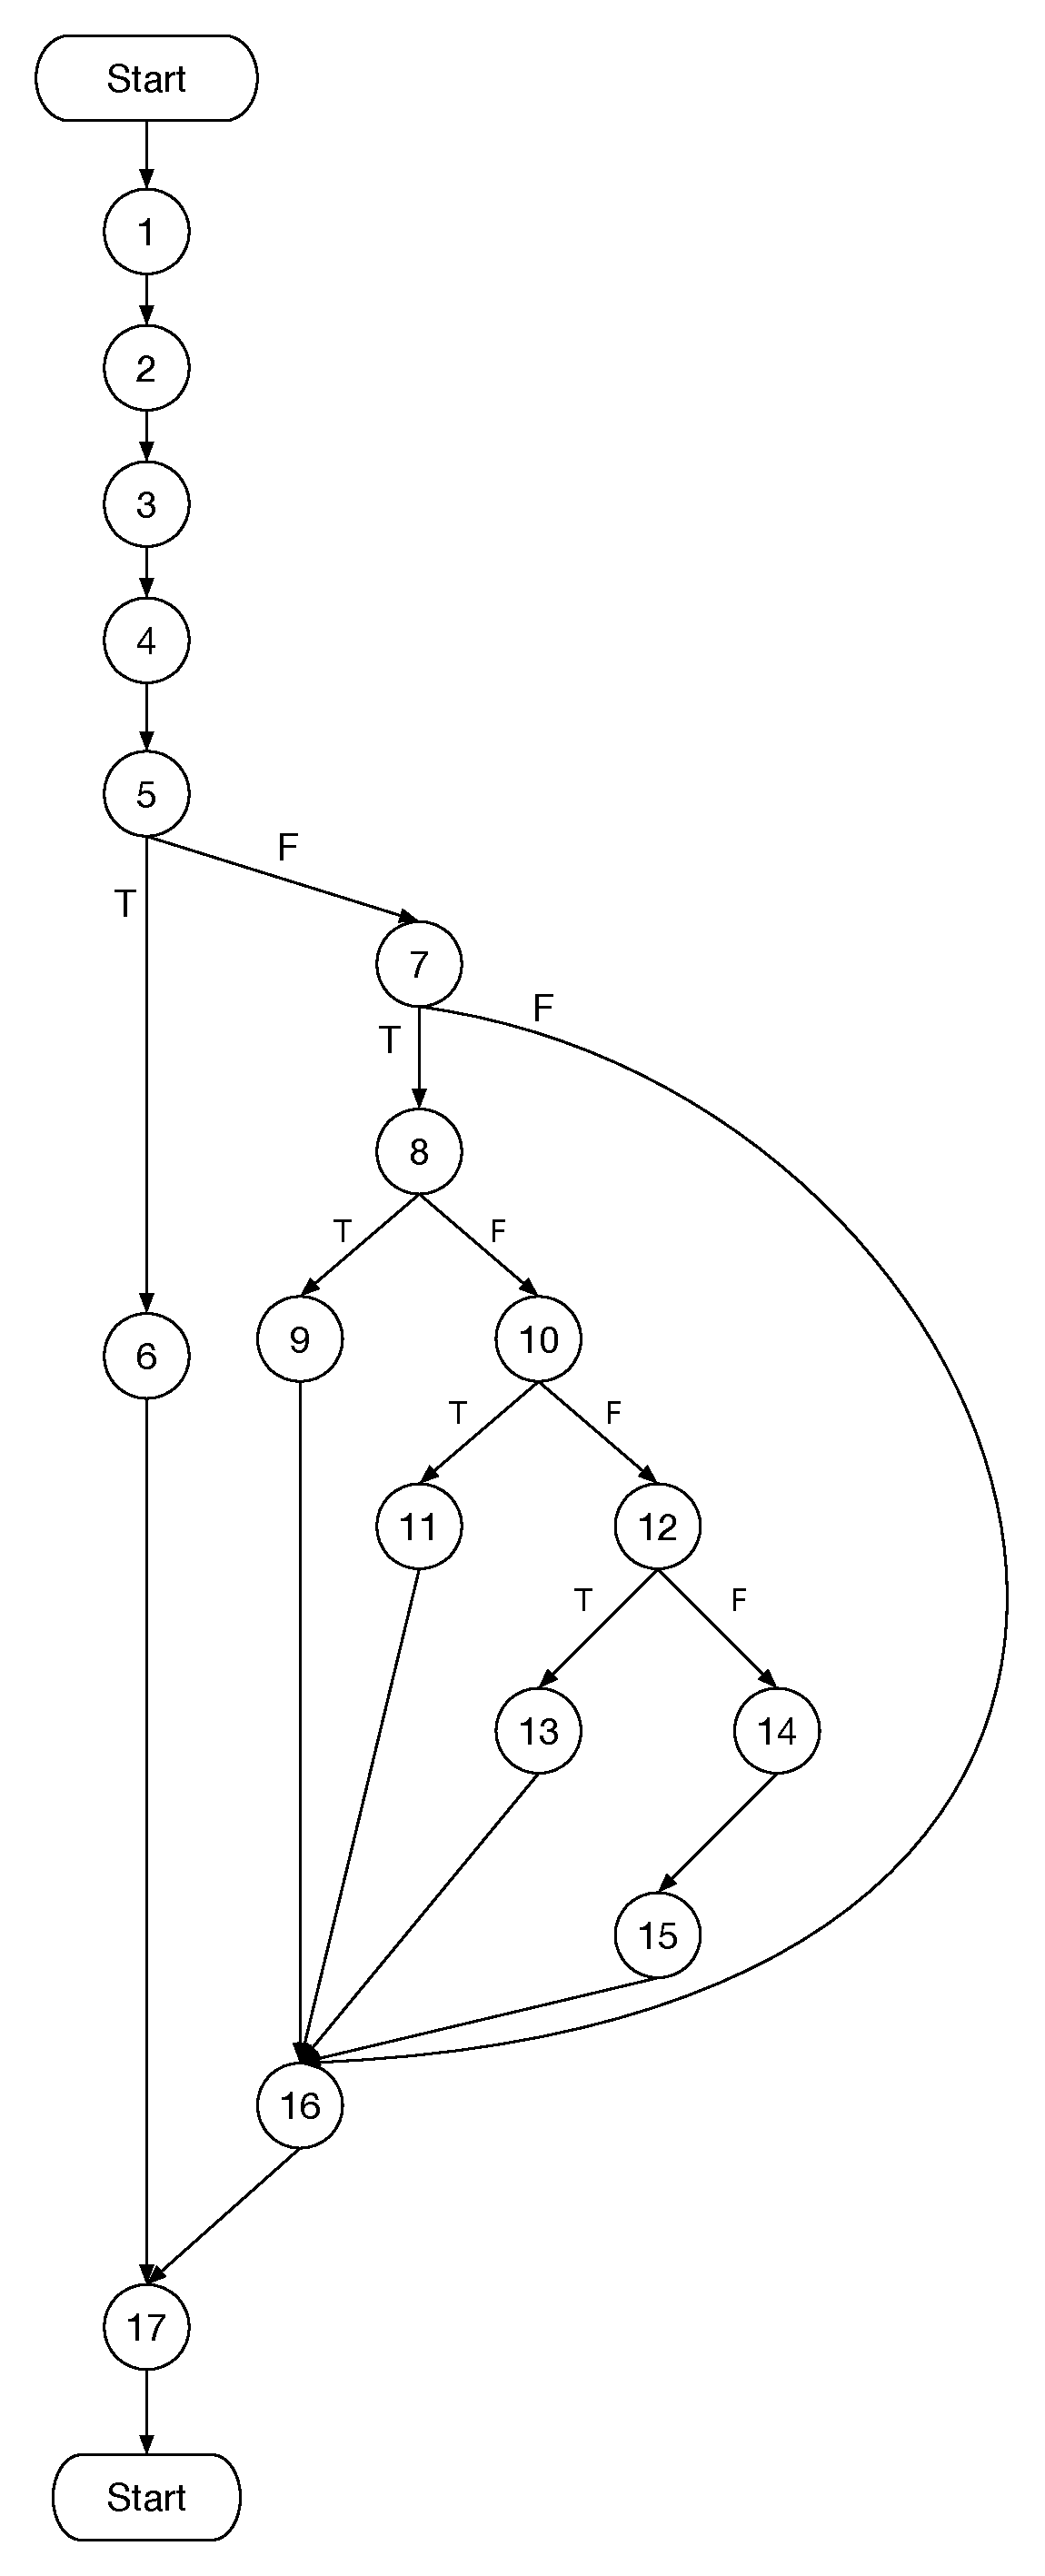
\includegraphics[height=0.8\textheight]{img/graph-testing-pythagorus.eps}
    \caption{Control flow graph ของโปรแกรมตรวจสอบรูปสามเหลี่ยมจาก \lstlistingname\, \ref{sec:trianglecal}}
\end{figure}

\newpage
% Coverage table
\clearpage
\begin{landscape}
    \section{Coverage table}
    จากกราฟใน~\numbername~\ref{fig:flowgraph} นำมาสร้าง Control Flow Graph ได้ดัง~\tablename~\ref{tab:coveragetable} ด้านล่าง
    \label{sec:coveragetable}
    \begin{table}[hb!]
        \caption{Coverage Table}
        \label{tab:coveragetable}
        \begin{center}
            % ID, Path, Decisionx3, Inputx3, Expected output = 9 cols
            \begin{tabular}[p]{ | c | l | *{8}{c|} l |}
                \hline
                \multirow{2}{*}{ID} & \multicolumn{1}{c}{\multirow{2}{*}{Path}} & \multicolumn{5}{|c|}{Decision} & \multicolumn{3}{|c|}{Inputs} & \multicolumn{1}{c|}{\multirow{2}{*}{Expected Output}} \\ \cline{3-10}
                                    &                                                   & 5  & 7  & 8  & 10 & 12 & a   & b   & c   &                \\ \hline
                1 & 1-2-3-4-5-6-18                                                      & T  & -  & -  & -  & -  & 201 & 201 & 201 & \outbound      \\ \hline
                2 & 1-2-3-4-$\bar{5}$-$\bar{7}$-16-17-18                                & F  & F  & -  & -  & -  & 100 &   1 &   1 & \nottriangle   \\ \hline
                3 & 1-2-3-4-$\bar{5}$-7-8-9-16-17-18                                    & F  & T  & T  & -  & -  & 100 & 100 & 100 & \equ           \\ \hline
                4 & 1-2-3-4-$\bar{5}$-7-$\bar{8}$-10-11-16-17-18                        & F  & T  & F  & T  & -  &   5 &   4 &   3 & \righttri      \\ \hline
                5 & 1-2-3-4-$\bar{5}$-7-$\bar{8}$-$\bar{10}$-12-13-16-17-18             & F  & T  & F  & F  & T  &   1 &   2 &   4 & \sca           \\ \hline
                6 & 1-2-3-4-$\bar{5}$-7-$\bar{8}$-$\bar{10}$-$\bar{12}$-14-15-16-17-18  & F  & T  & F  & F  & F  & 100 & 100 &  50 & \iso           \\ \hline
            \end{tabular}
        \end{center}
    \end{table}

\end{landscape}
\end{document}
